\subsection*{Task 2}

\subsubsection*{c)}

\begin{figure}[h!]
  \centering
  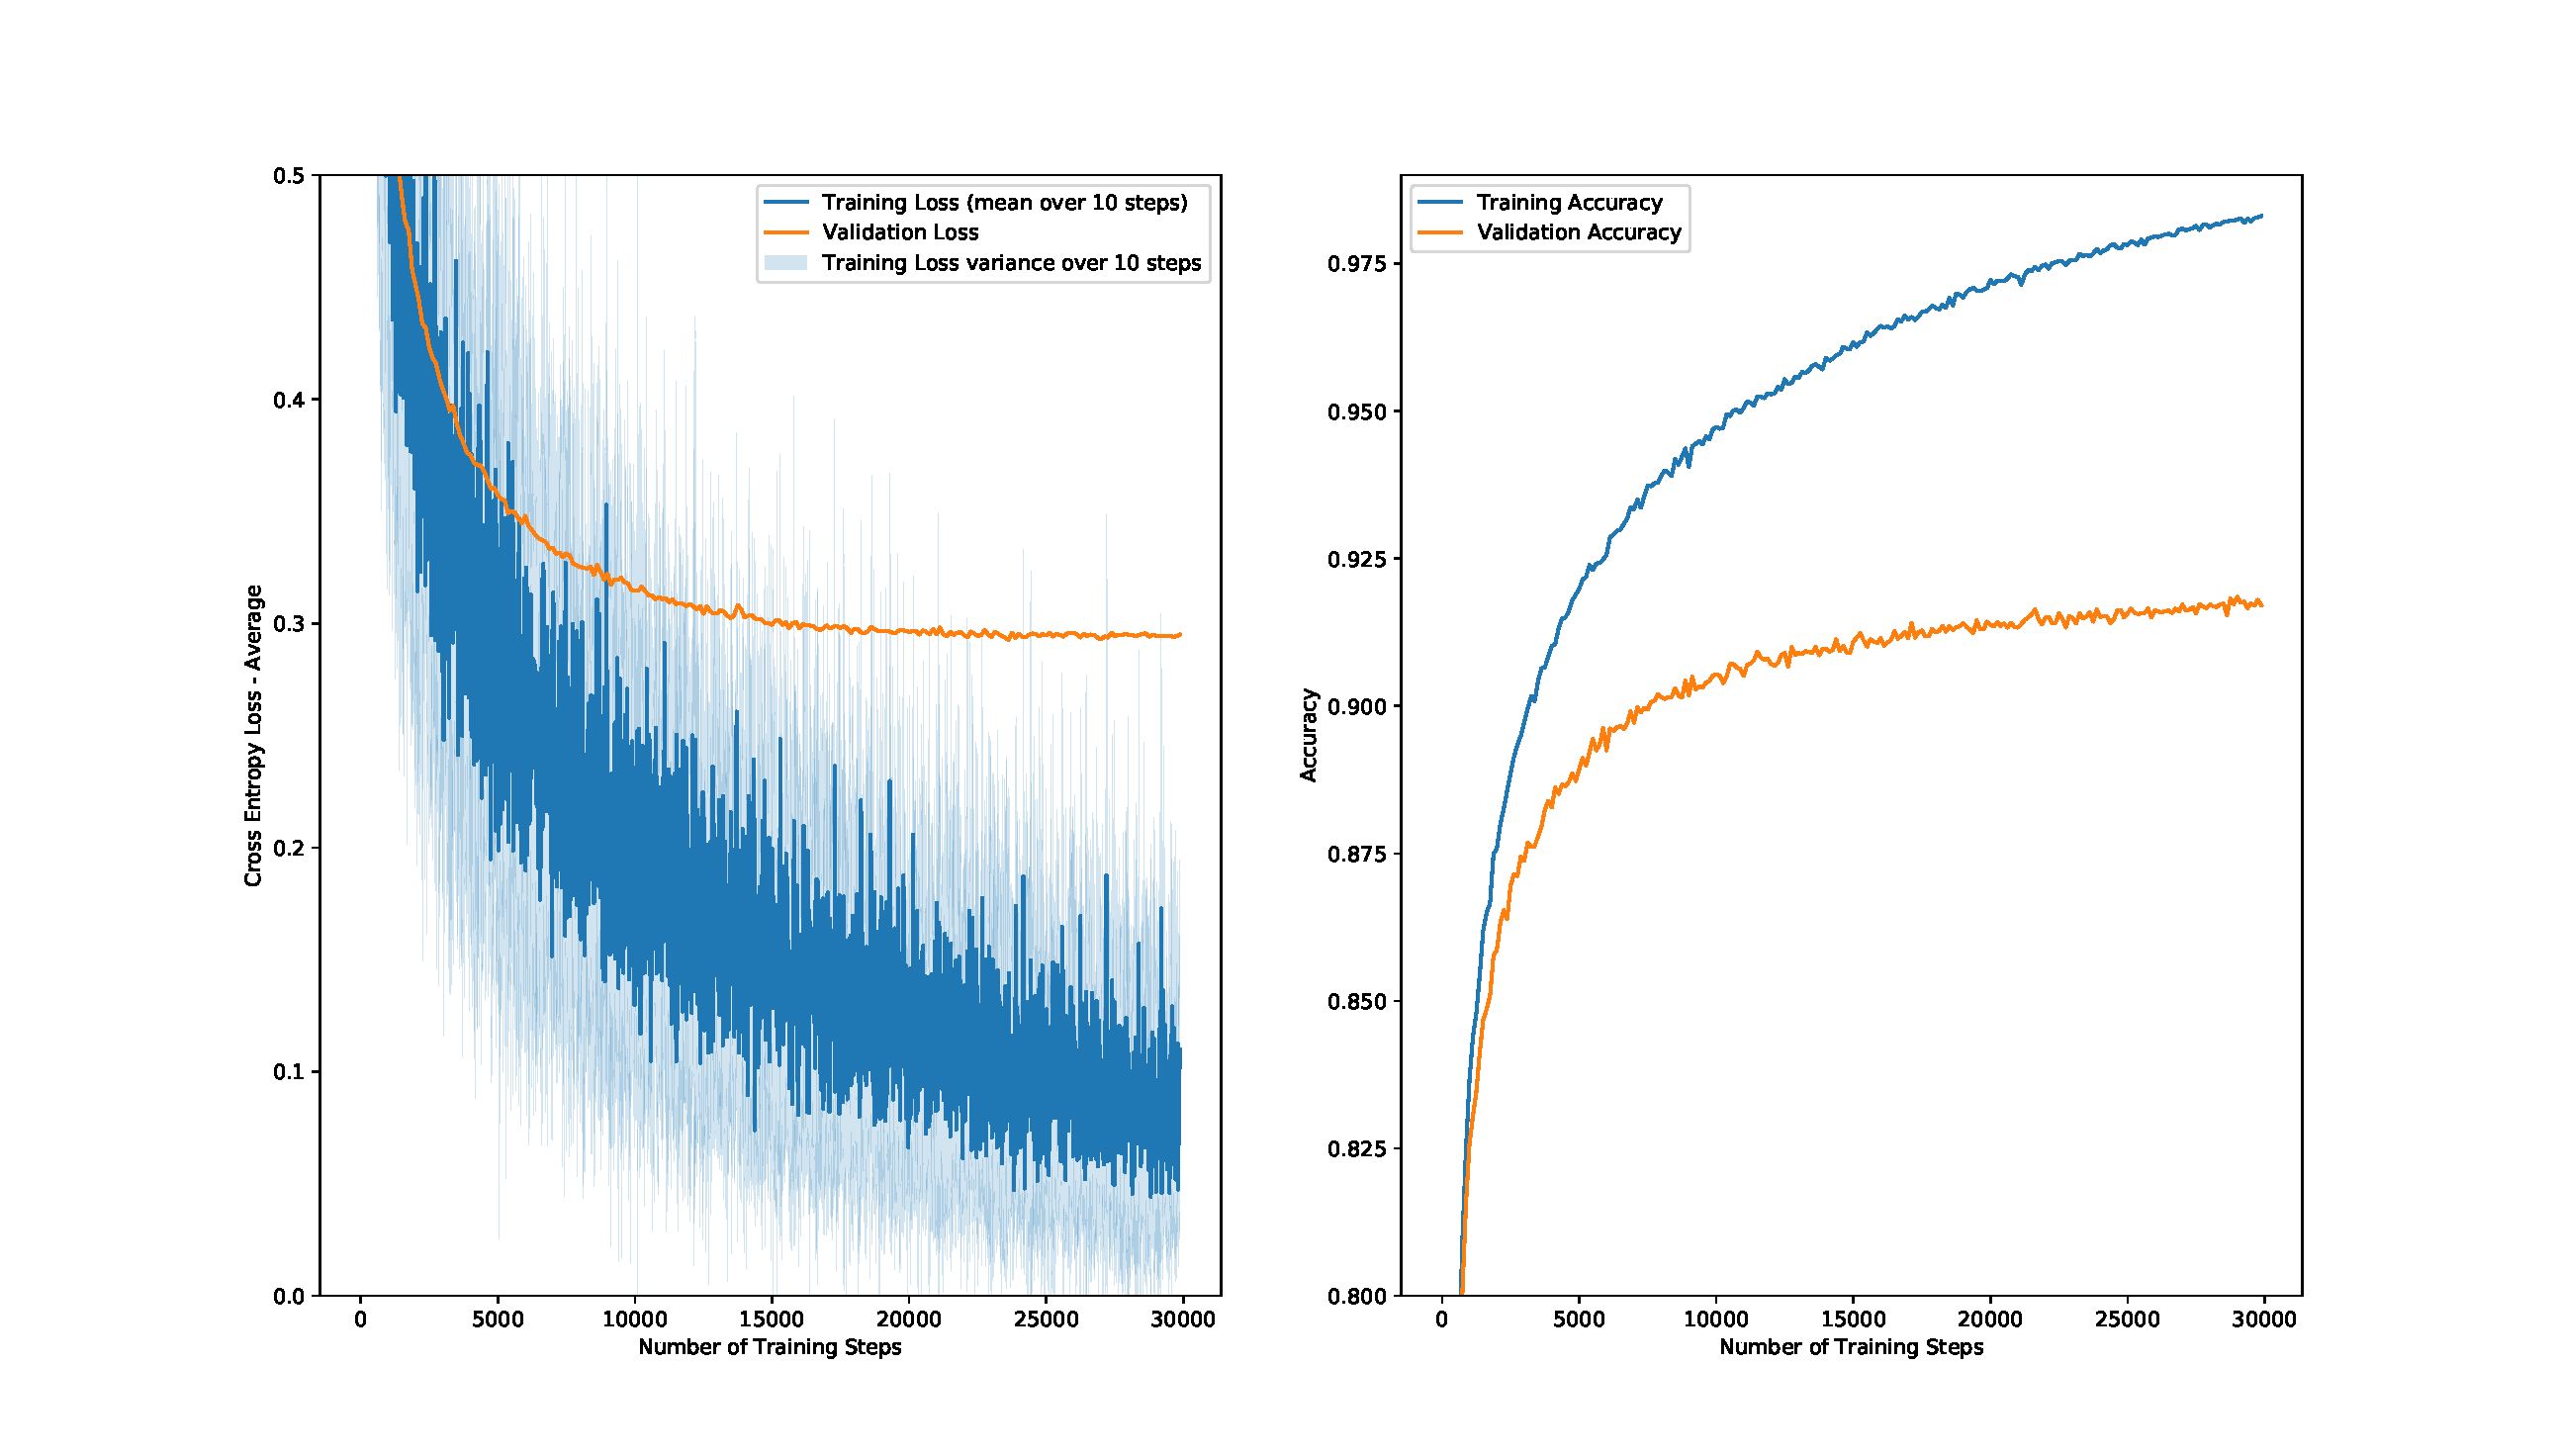
\includegraphics[clip, trim=3cm 0cm 3cm 0cm ,width=\textwidth]{figures/Task2c.pdf}
  \caption{Training and validation set loss (left) and accuracy (right) over training.}
  \label{fig:task2:loss_accuracy}
\end{figure}


\subsubsection*{d)}

We have 785 input nodes, 64 hidden nodes and 10 output nodes, giving a total of $785 \times 64 + 64 \times 10 = 50880$ parameters in the network.
